\chapter{Architekturschichten}\label{ch:arrchitekturschichten}
Im Folgenden wird die Architektur der Applikation genauer beschrieben. Dabei liegt das Augenmerk 
auf der Struktur, dem Verhalten und der Verteilung der einzelnen Komponenten in der Architektur.

%Einzelne Unterkategorien werden ergänzt, wenn die Implementierung der Applikation voran schreitet.

\section{Strukturschicht}\label{sec:strukturschicht}
% ,angle=90,origin=c

\subsection{Backend}
In diesem Abschnitt ist die Struktur des Backends beschrieben.

\begin{figure}[H]
    \centering
    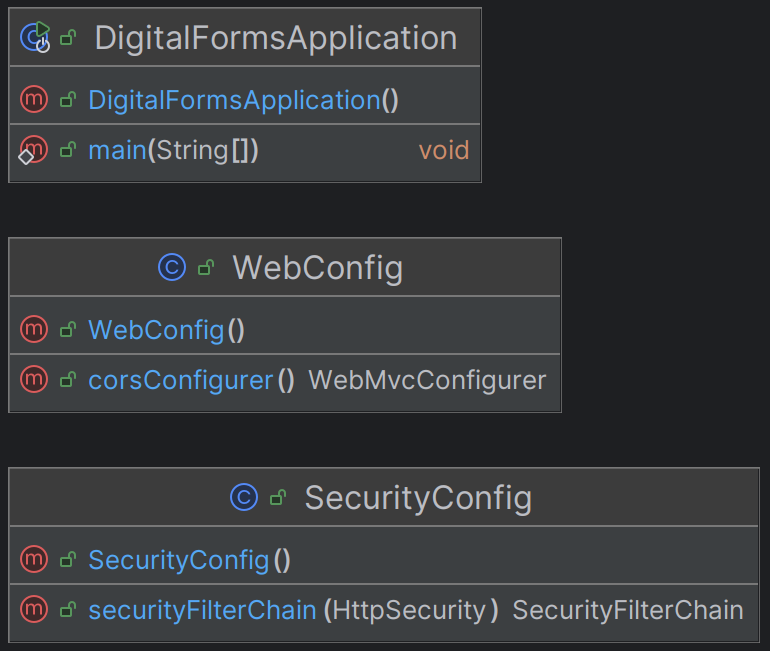
\includegraphics[width=15cm]{images/classDiagrams/Config}
    \caption{Backend Spring Boot Configuration}\label{fig:Backend-Spring-Boot-Configuration}
\end{figure}

\refa{fig:Backend-Spring-Boot-Configuration} zeigt die Konfiguration des Spring Boot Projekts.
Dabei startet "DigitalFormsApplication" das Projekt, "WebConfig" Konfiguriert CORS Einstellungen und "SecurityConfig"
Konfiguriert die Zugriffsoptionen auf die Endpunkte.

\begin{figure}[H]
    \centering
    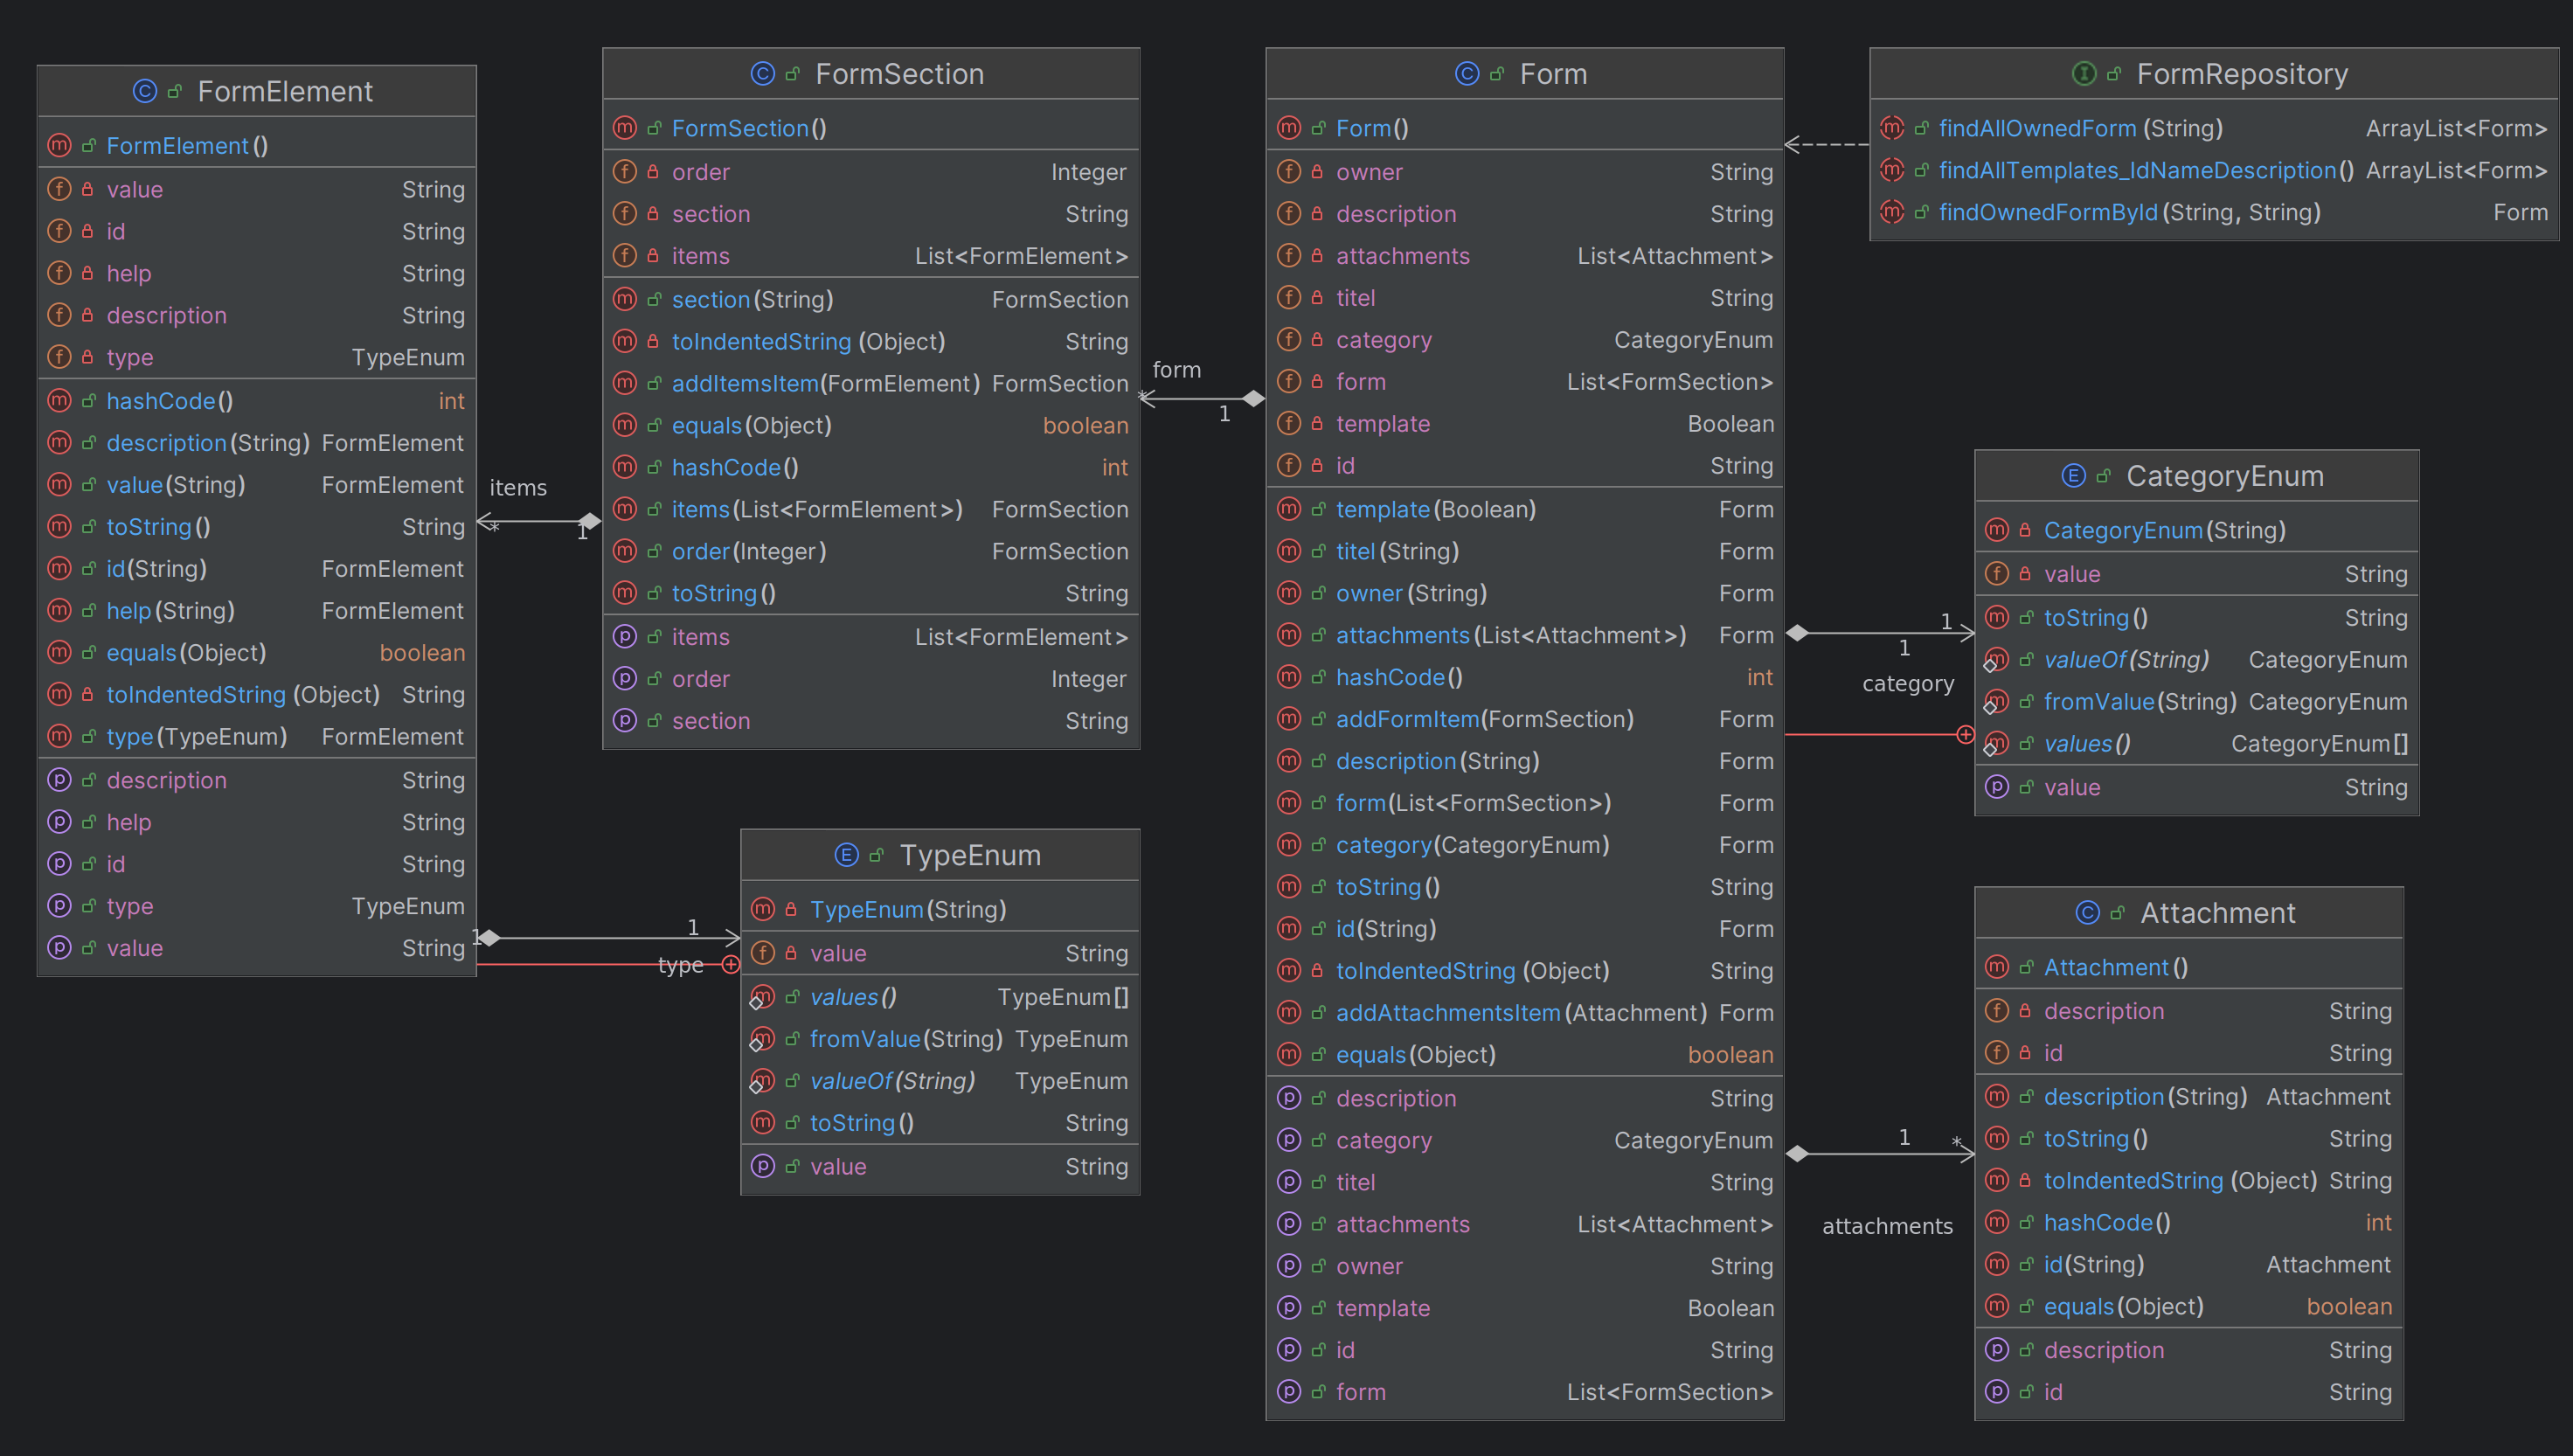
\includegraphics[width=20cm,angle=90,origin=c]{images/classDiagrams/FormRepository}
    \caption{Backend Datenmodell}\label{fig:backendclass-diagram}
\end{figure}

\refa{fig:backendclass-diagram} zeigt den detailarten Aufbau des Datenbank modells.
Dabei dient "FormRepository" als Schnittstelle für die Datenbank.
Die Objektmodelle werden durch die OpenAPI Spezifikation automatisch generiert.

\begin{figure}[H]
    \centering
    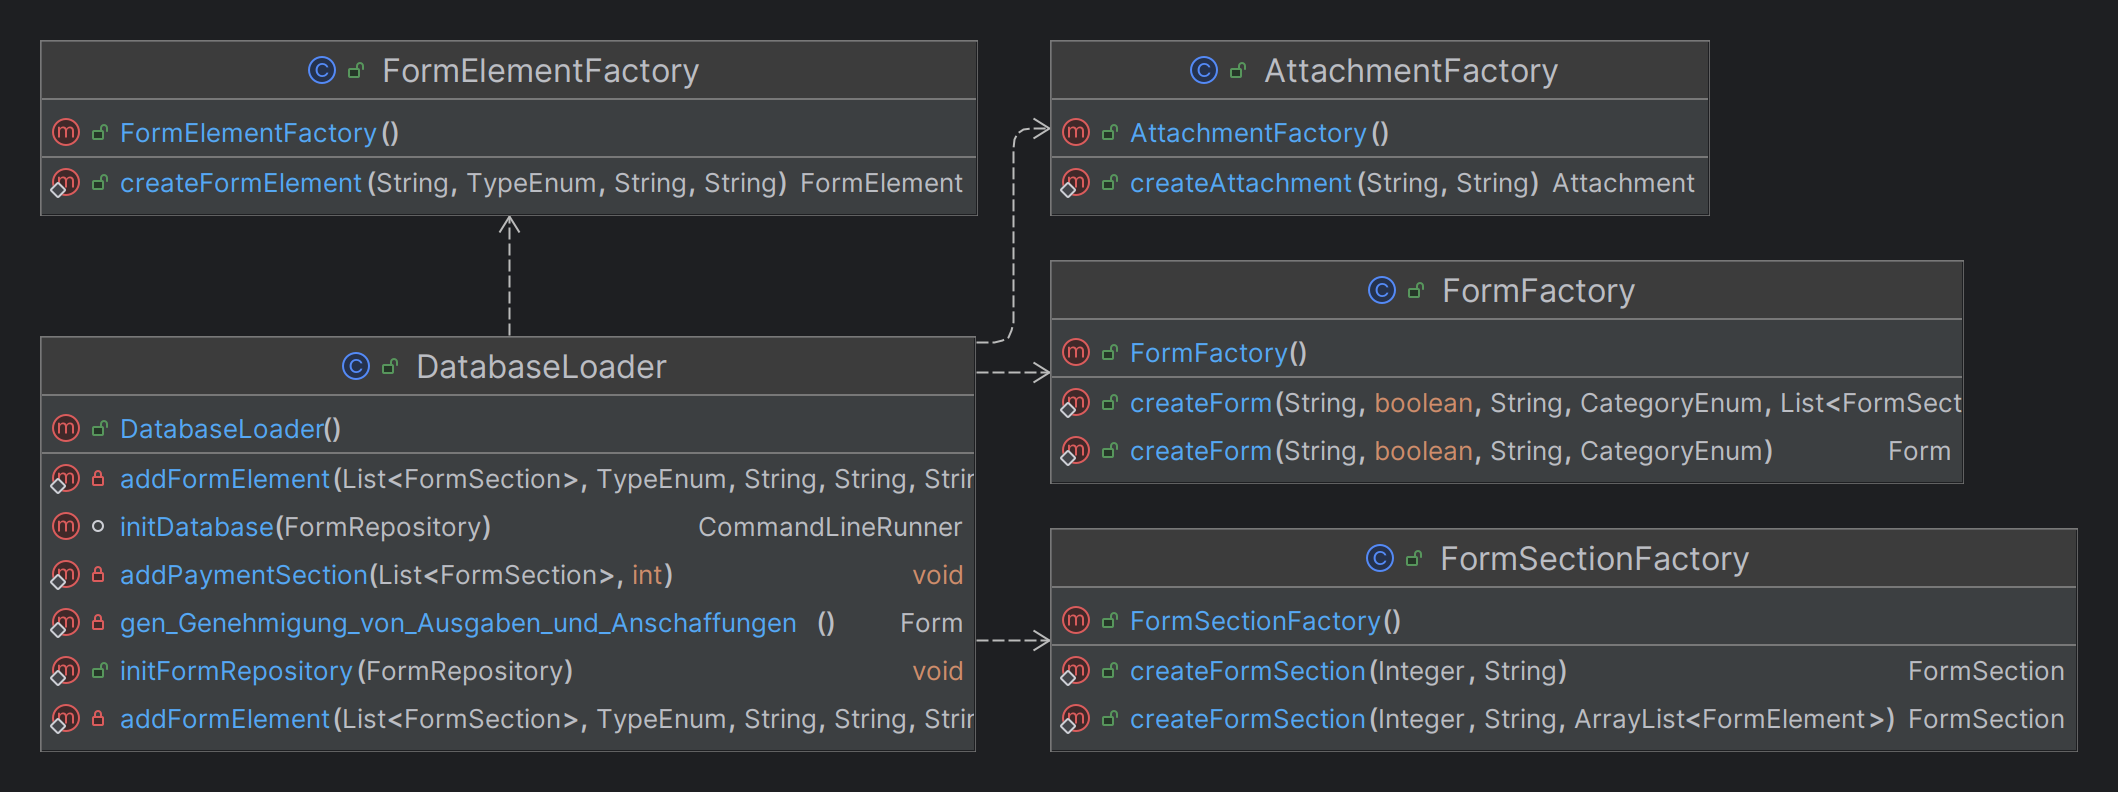
\includegraphics[width=15cm]{images/classDiagrams/DatabaseLoader}
    \caption{Backend Datenbank Init und Factorys}\label{fig:backend-gen-class-diagram}
\end{figure}

Um die Datenbank mit Elementen zu initialisieren wird der "DatabaseLoader" aus \refa{fig:backend-gen-class-diagram}.
Dieser generiert mithilfe von Factories Elemente für die Datenbank.

\begin{figure}[H]
    \centering
    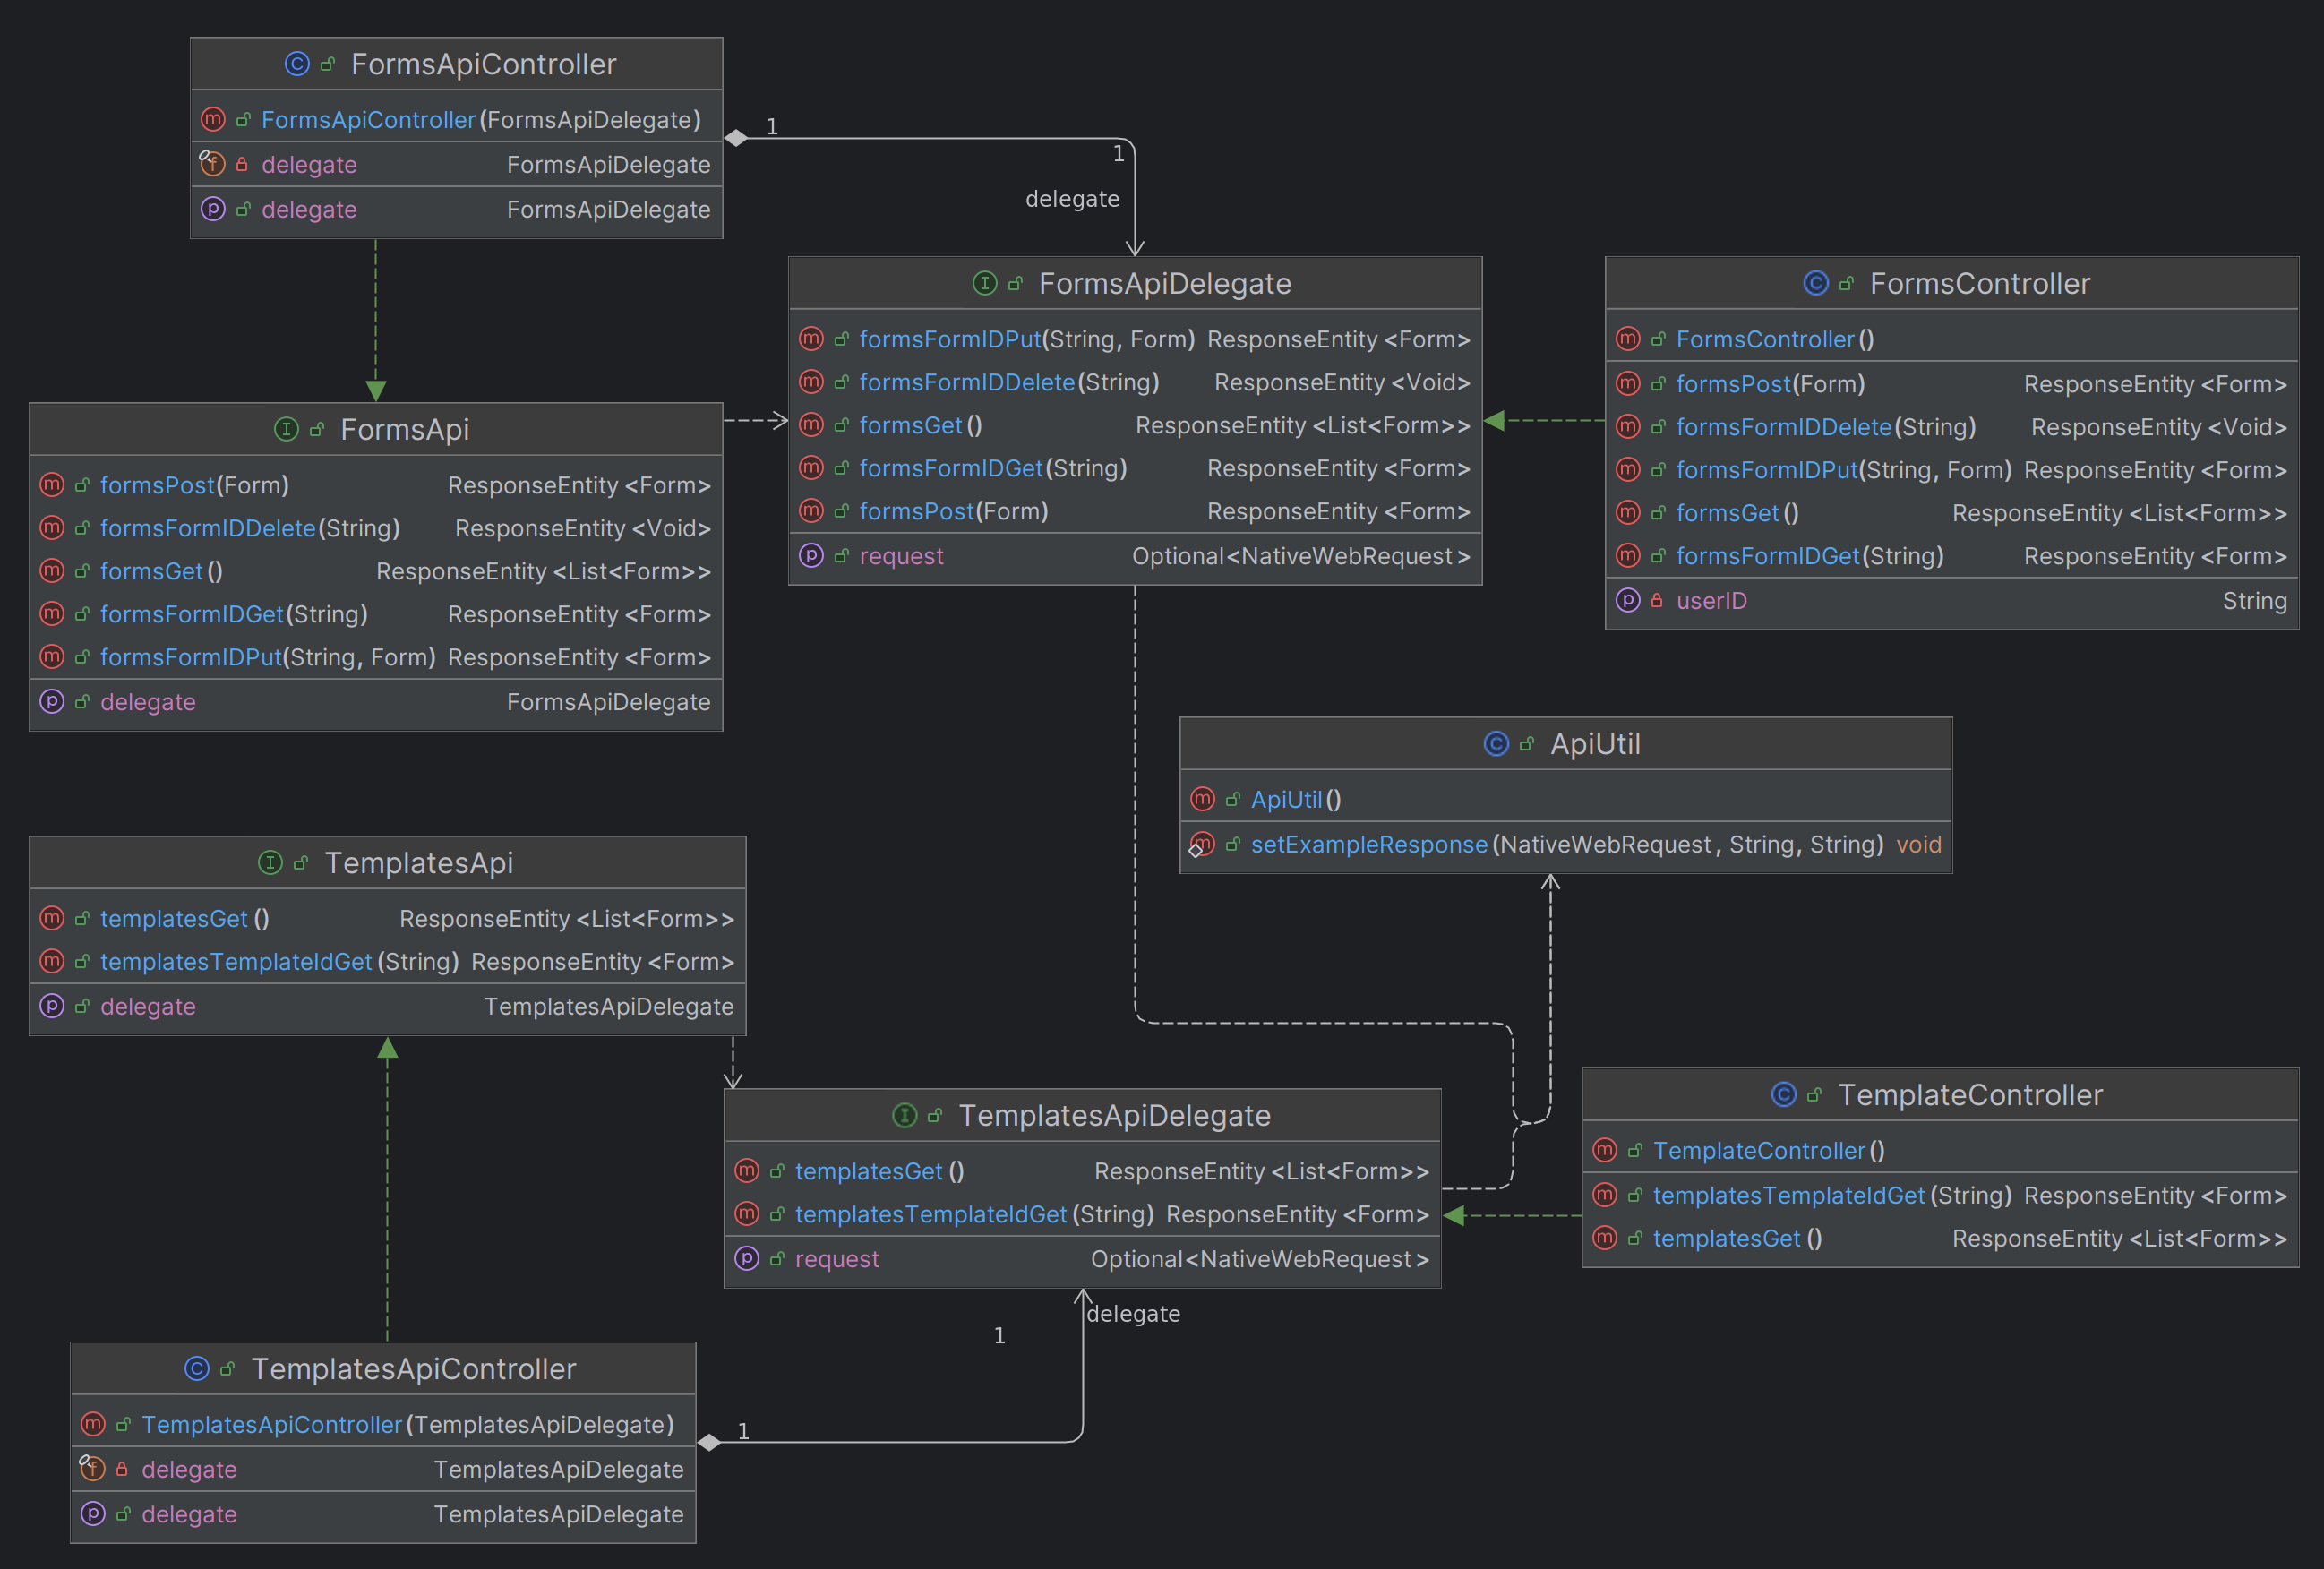
\includegraphics[width=15cm]{images/classDiagrams/Api}
    \caption{Backend API Controller}\label{fig:Backend-API-Controller}
\end{figure}

Die Implementierung der \ac{API} Endpunkte erfolgt in den jeweiligen Controllern.
Diese verwenden generierte Interfaces wie in \refa{fig:Backend-API-Controller} zu sehen ist.

% \subsection{Frontend}
% Irgendwie Unhappy damit
% Finde Beim Frontend Derzeit nichts Sinfolles

\section{Verhaltensschicht}\label{sec:verhaltensschicht}
Im Folgenden wird das Verhalten der Applikation bei verschiedenen Usecases beschrieben.

\section{Verteilungsschicht}\label{sec:verteilungsschicht}
Die feingranulare Verteilung von Funktionalitäten in unserer Applikation sieht wie folgt aus:

\begin{figure}[h]
    \centering
    \includesvg[width=15cm]{./images/GeneralNetwork}
    \caption{Netzwerksübersicht}\label{fig:Netzwerksuebersicht}
\end{figure}




\begin{figure}[h]
    \centering
    \includesvg[width=15cm]{images/ServerSetup}
    \caption{Container verteilung}\label{fig:Container-verteilung}
\end{figure}